\documentclass[11pt]{standalone}
\usepackage{amssymb}
\usepackage{amsmath}
\usepackage[no-math]{fontspec}
\usepackage{unicode-math}
\usepackage{libertinus}
\usepackage{pgf,xcolor}
\usepackage{tikz}
\usetikzlibrary{arrows.meta, backgrounds}
\usepackage{pgfplots}
\pgfplotsset{compat=newest}

\definecolor{my_darkgray}{HTML}{484949}
\definecolor{my_lightgray}{HTML}{F3F4F4}
\definecolor{my_darkblue}{HTML}{005A94}
\definecolor{my_lightblue}{HTML}{CCDEE9}
\definecolor{my_yellow}{HTML}{FFEC7F}
\definecolor{my_red}{HTML}{E60000}
\definecolor{my_orange}{HTML}{E87846}

\begin{document}
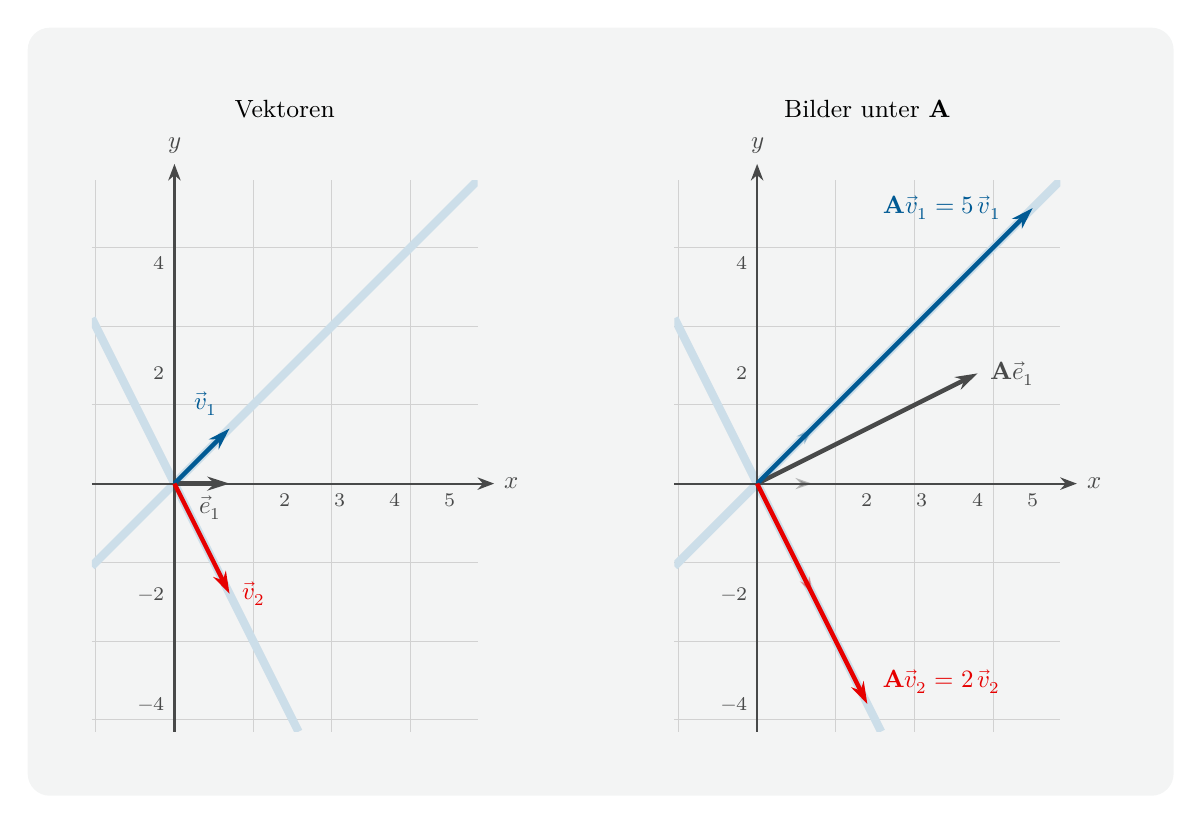
\begin{tikzpicture}[
    show background rectangle,
    background rectangle/.style={fill=my_lightgray, rounded corners=8pt},
    inner frame sep=0.8cm,
    x=0.7cm, y=0.7cm,
    vec/.style={-{Stealth[length=8pt, width=5pt]}, ultra thick},
    alt/.style={-{Stealth[length=6pt, width=4pt]}, thick, opacity=0.35}
]

% ---------------------------------------------------------------
%  A = (4 1; 2 3) mit den Eigenvektoren
%    v1 = (1, 1)   zum Eigenwert 5:  A v1 = (5, 5)
%    v2 = (1, -2)  zum Eigenwert 2:  A v2 = (2, -4)
%  Gegenbeispiel e1 = (1, 0):        A e1 = (4, 2)
%  Beide Teilbilder im selben Massstab und Ausschnitt.
% ---------------------------------------------------------------

\newcommand{\gitter}{
    \draw[my_darkgray!25, thin] (-1.5, -4.5) grid (5.5, 5.5);
    % Geraden durch die Eigenvektoren
    \begin{scope}
        \clip (-1.5, -4.5) rectangle (5.5, 5.5);
        \draw[my_lightblue, line width=3pt] (-1.5, -1.5) -- (5.5, 5.5);
        \draw[my_lightblue, line width=3pt] (-1.5, 3) -- (2.25, -4.5);
    \end{scope}
    \draw[-{Stealth[length=6pt]}, thick, my_darkgray] (-1.5, 0) -- (5.8, 0)
        node[right, font=\small] {$x$};
    \draw[-{Stealth[length=6pt]}, thick, my_darkgray] (0, -4.5) -- (0, 5.8)
        node[above, font=\small] {$y$};
    \foreach \x in {2, ..., 5}
        \node[below, font=\scriptsize, my_darkgray] at (\x, 0) {$\x$};
    \foreach \y in {-4, -2, 2, 4}
        \node[left, font=\scriptsize, my_darkgray] at (0, \y) {$\y$};
}

% ===== Linkes Teilbild: die Vektoren =====
\begin{scope}
    \gitter

    \draw[vec, my_darkgray] (0, 0) -- (1, 0);
    \node[below, font=\small, my_darkgray] at (0.65, -0.05) {$\vec{e}_1$};
    \draw[vec, my_darkblue] (0, 0) -- (1, 1);
    \node[above left, font=\small, my_darkblue] at (0.95, 1.05) {$\vec{v}_1$};
    \draw[vec, my_red] (0, 0) -- (1, -2);
    \node[right, font=\small, my_red] at (1.05, -2) {$\vec{v}_2$};

    \node[font=\small] at (2, 6.8) {Vektoren};
\end{scope}

% ===== Rechtes Teilbild: ihre Bilder unter A =====
\begin{scope}[xshift=7.4cm]
    \gitter

    % Ausgangsvektoren zum Vergleich
    \draw[alt, my_darkgray] (0, 0) -- (1, 0);
    \draw[alt, my_darkblue] (0, 0) -- (1, 1);
    \draw[alt, my_red] (0, 0) -- (1, -2);

    \draw[vec, my_darkgray] (0, 0) -- (4, 2);
    \node[right, font=\small, my_darkgray] at (4.05, 2) {$\mathbf{A}\vec{e}_1$};
    \draw[vec, my_darkblue] (0, 0) -- (5, 5);
    \node[left, font=\small, my_darkblue] at (4.6, 5) {$\mathbf{A}\vec{v}_1 = 5\,\vec{v}_1$};
    \draw[vec, my_red] (0, 0) -- (2, -4);
    \node[right, font=\small, my_red] at (2.1, -3.6) {$\mathbf{A}\vec{v}_2 = 2\,\vec{v}_2$};

    \node[font=\small] at (2, 6.8) {Bilder unter $\mathbf{A}$};
\end{scope}

\end{tikzpicture}
\end{document}
